\documentclass[12pt]{article}

\usepackage{amsmath, amssymb, amsthm, enumerate, graphicx}
\usepackage[usenames,dvipsnames]{color}
\usepackage{bm}
\usepackage[colorlinks=true,urlcolor=blue]{hyperref}
\usepackage{geometry}
\geometry{margin=1in}
\usepackage{float}
\usepackage{graphics}
\setlength{\marginparwidth}{2.15cm}
\usepackage{booktabs}
\usepackage{enumitem}
\usepackage{epsfig}
\usepackage{setspace}
\usepackage{parskip}
\usepackage[normalem]{ulem}
\usepackage{tikz}
\usetikzlibrary{positioning, arrows, automata}
\usepackage{pgfplots}
\usepackage[font=scriptsize]{subcaption}
\usepackage{float}
\usepackage[]{algorithm2e}
\usepackage{environ}
\usepackage{bbm}
\usepackage{graphicx}
\usepackage{titling}
\usepackage{url}
\usepackage{xcolor}
\usepackage{lipsum}
\usepackage{lastpage}
\usepackage[colorlinks=true,urlcolor=blue]{hyperref}
\usepackage{multicol}
\usepackage{tabularx}
\usepackage{comment}
\usepackage[utf8]{inputenc}
\usepackage{amssymb}
\usepackage{setspace}
\usepackage{marvosym}
\usepackage{wrapfig}
\usepackage{datetime}
\usepackage[many]{tcolorbox}
\usepackage{array}
\usepackage{multirow}
\usepackage{wasysym}
\usepackage{cancel}

\usepackage{listings}
\usepackage{color}
\usepackage[thinlines]{easytable}
\usepackage{lastpage}

\newcommand{\R}{\mathbb{R}}
\newcommand{\blackcircle}{\tikz\draw[black,fill=black] (0,0) circle (1ex);}
\renewcommand{\circle}{\tikz\draw[black] (0,0) circle (1ex);}


\usetikzlibrary{positioning,calc}


%-------------------------------------------------------------------------------
% Custom commands
\usepackage{xcolor} %hilight
\newcommand{\hilight}[1]{\colorbox{yellow}{#1}}
%-------------------------------------------------------------------------------

\newtcolorbox[]{solution}[1][]{%
    breakable,
    enhanced,
    colback=white,
    title=Solution,
    #1
}
\begin{document}
\section*{}
\begin{center}
  \centerline{\textsc{\LARGE  Homework 4 Submission}}
\end{center}

Use this template to record your answers for Homework 4.  Add your answers using \LaTeX and then save your document as a PDF to upload to Gradescope.  You are required to use this template to submit your answers.  \textbf{You should not alter this template in any way} other than to insert your solutions.  You must submit all \pageref{LastPage} pages of this template to Gradescope.  Do not remove the instructions page(s).  Altering this template or including your solutions outside of the provided boxes can result in your assignment being graded incorrectly.

You should also export your code as a .py file and upload it to the \textbf{separate} Gradescope coding assignment. Remember to mark all teammates on \textbf{both} assignment uploads through Gradescope.

\section*{Instructions for Specific Problem Types}

On this homework, you must fill in blanks for each problem. Please make sure your final answer is fully included in the given space.  \textbf{Do not change the size of the box provided.}  For short answer questions you should \textbf{not} include your work in your solution.  Only provide an explanation or proof if specifically asked.

\begin{quote}
\textbf{Fill in the blank:} What is the course number?

\begin{tcolorbox}[fit,height=1cm, width=4cm, blank, borderline={1pt}{-2pt},nobeforeafter]
    \begin{center}\huge10-703\end{center}
    \end{tcolorbox}
\end{quote}

\newpage

\section*{Problem 0: Collaborators}
Enter your team members' names and Andrew IDs in the boxes below. If you worked in a team with fewer than three people, leave the extra boxes blank.

Name 1: \begin{tcolorbox}[fit,height=1cm, width=5cm, blank, borderline={1pt}{1pt},nobeforeafter]
    \begin{center}
    \vspace{3mm}
    \large{Arnav Goyal}
    \end{center}
\end{tcolorbox}
Andrew ID 1: \begin{tcolorbox}[fit,height=1cm, width=5cm, blank, borderline={1pt}{1pt},nobeforeafter]
    \begin{center}
    \vspace{3mm}
    \large{arnavgoy}
    \end{center}
\end{tcolorbox}
    \\
Name 2: \begin{tcolorbox}[fit,height=1cm, width=5cm, blank, borderline={1pt}{1pt},nobeforeafter]
    \begin{center}
    \vspace{3mm}
    \large{Vineeth Bhat}
    \end{center}
\end{tcolorbox}
Andrew ID 2: \begin{tcolorbox}[fit,height=1cm, width=5cm, blank, borderline={1pt}{1pt},nobeforeafter]
    \begin{center}
    \vspace{3mm}
    \large{vineethb}
    \end{center}
\end{tcolorbox} \\
Name 3: \begin{tcolorbox}[fit,height=1cm, width=5cm, blank, borderline={1pt}{1pt},nobeforeafter]
    \begin{center}
    \vspace{3mm}
    \large{Kushal Kejriwal}
    \end{center}
\end{tcolorbox}
Andrew ID 3: \begin{tcolorbox}[fit,height=1cm, width=5cm, blank, borderline={1pt}{1pt},nobeforeafter]
    \begin{center}
    \vspace{3mm}
    \large{kkejriwa}
    \end{center}
\end{tcolorbox} \\
\vspace{0.5cm}
\vspace{0.5cm}

\newpage
\section*{Problem 1: CMA-ES (24 pts)}
\subsection*{1.1 Plot of CMA-ES on simple objective function (10 pts)}
\begin{tcolorbox}[fit,height=30em, width=40em, blank, borderline={1pt}{1pt},nobeforeafter]
            \begin{center}
            \begin{solution}

            \end{solution}
            \end{center}
            \end{tcolorbox}
            
\subsection*{1.2 RL reward of fixed policies (4 pts)}

$x = (-1, -1, -1, -1, -1)$ : \begin{tcolorbox}[fit,height=1cm, width=5cm, blank, borderline={1pt}{1pt},nobeforeafter]
    \begin{center}
    \vspace{3mm}
    \large{15.6}
    \end{center}
\end{tcolorbox} \\
$x = (1, 0, 1, 0, 1)$ : \hspace{3.5em} \begin{tcolorbox}[fit,height=1cm, width=5cm, blank, borderline={1pt}{1pt},nobeforeafter]
    \begin{center}
    \vspace{3mm}
    \large{}
    \end{center}
\end{tcolorbox} \\
$x = (0, 1, 2, 3, 4)$ : \hspace{3.5em} \begin{tcolorbox}[fit,height=1cm, width=5cm, blank, borderline={1pt}{1pt},nobeforeafter]
    \begin{center}
    \vspace{3mm}
    \large{}
    \end{center}
\end{tcolorbox}

\subsection*{1.3 Plot of CMA-ES on Cartpole (10 pts)}
\begin{tcolorbox}[fit,height=30em, width=40em, blank, borderline={1pt}{1pt},nobeforeafter]
    \begin{center}
    \begin{solution}

    \end{solution}
    \end{center}
    \end{tcolorbox}
    
\newpage

\subsection*{Problem 2: Imitation Learning (62 pts)}
\subsection*{Problem 2.1: BC (14 pts)}

\subsection*{2.1.1 Loss Plot + Final Loss Value BC (6 pts)}
\begin{tcolorbox}[fit,height=20em, width=40em, blank, borderline={1pt}{1pt},nobeforeafter]
            \begin{solution}                  
            \centering
            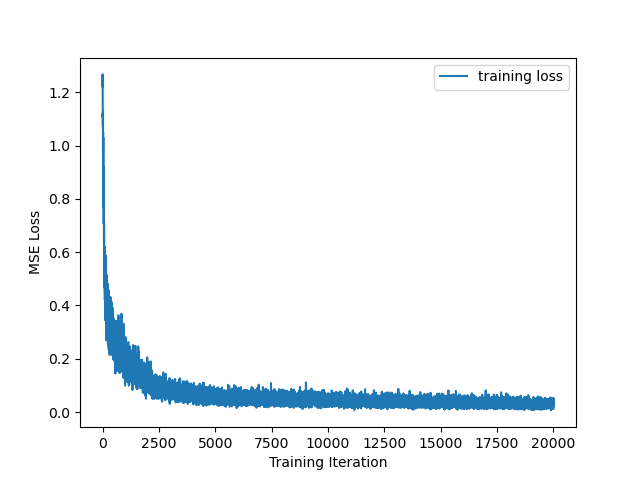
\includegraphics[width=21.5em]{code/results_BC/trial_2_BEST/BC_losses.png}

            Final loss: 0.0123

                                    \end{solution}
            \end{tcolorbox}

\subsection*{2.1.2 Rewards Plot BC (6 pts)}

\begin{tcolorbox}[fit,height=24em, width=40em, blank, borderline={1pt}{1pt},nobeforeafter]
            \begin{solution}
            \centering
            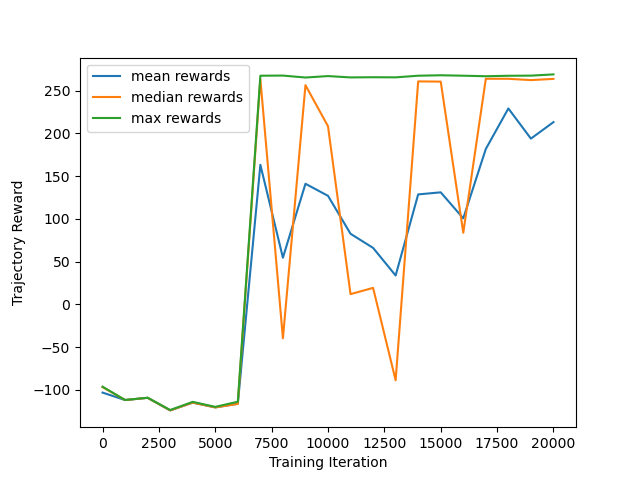
\includegraphics[width=27em]{code/results_BC/trial_2_BEST/BC_rewards.png}

                                \end{solution}

\end{tcolorbox}
\subsection*{2.1.3 GIF link BC (2 pts)}

\begin{tcolorbox}[fit,height=5em, width=40em, blank, borderline={1pt}{1pt},nobeforeafter]
            \begin{solution}
            \url{https://drive.google.com/file/d/1Z3-S1BLQdJrHZxqDcdyWtXMBsSGnJxWQ/view?usp=sharing}
            \end{solution}

\end{tcolorbox}

\subsection*{Problem 2.2: DAgger (18 pts)}

\subsection*{2.2.1 Loss Plot DAgger (6 pts)}
\begin{tcolorbox}[fit,height=20em, width=40em, blank, borderline={1pt}{1pt},nobeforeafter]
            \begin{center}
            \begin{solution}                    
            \centering
            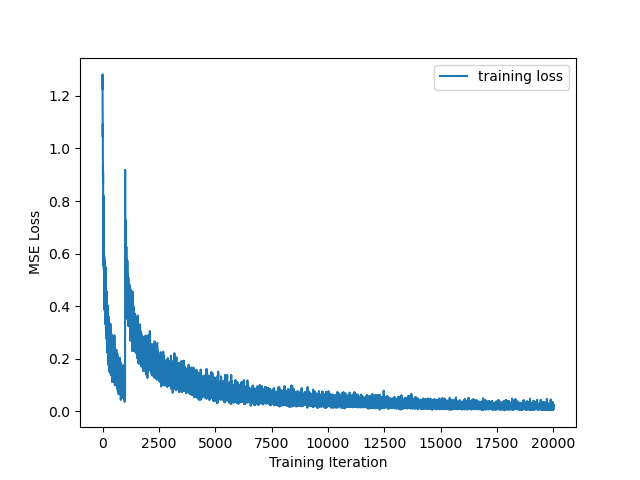
\includegraphics[width=21.5em]{code/results_DAgger/trial_3_BEST/DAgger_losses.png}

            Final loss: 0.0168
            
                        \end{solution}
            \end{center}
            \end{tcolorbox}
           
            
\subsection*{2.2.2 Rewards Plot DAgger (6 pts)}

\begin{tcolorbox}[fit,height=24em, width=40em, blank, borderline={1pt}{1pt},nobeforeafter]
            \begin{center}
            \begin{solution}
            \centering
            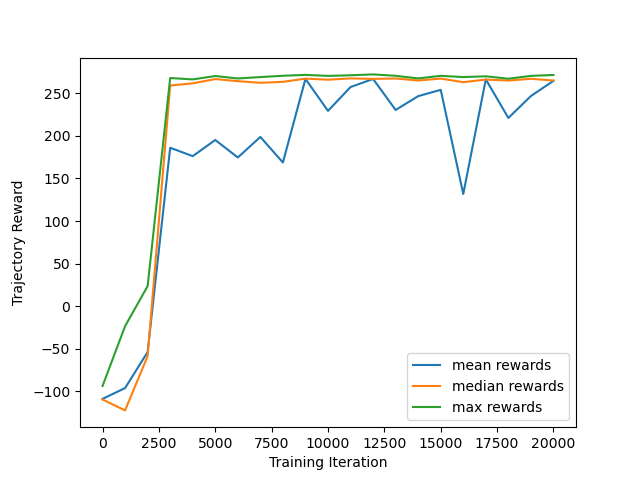
\includegraphics[width=27em]{code/results_DAgger/trial_3_BEST/DAgger_rewards.png}

            \end{solution}
\end{center}
\end{tcolorbox}

\subsection*{2.2.3 GIF link DAgger (2 pts)}

\begin{tcolorbox}[fit,height=5em, width=40em, blank, borderline={1pt}{1pt},nobeforeafter]
            \begin{solution}
            \url{https://drive.google.com/file/d/1Tz_Nix4edSxUjCrV3Y8WdhgI3HLD5d7Q/view?usp=sharing}
            \end{solution}

\end{tcolorbox}

\subsection*{2.2.4 Compare DAgger training with BC (written, 4 pts)}
\begin{tcolorbox}[fit,height=10em, width=40em, blank, borderline={1pt}{1pt},nobeforeafter]
            \begin{center}
            \begin{solution}
            \raggedright
DAgger worked better. We did 5 independent runs over both DAgger and plain BC, and we observed that we learned how to 
walk in all 5 DAgger runs (final mean reward 240–265; close to expert's 261–266) while only in 3 of the BC runs (final mean reward 193–213), despite similar training losses.
BC only sees states from expert trajectories, so a small action error takes the walker to states the expert never visited,
where its errors compound until it falls. With per-step error $\epsilon$ over horizon $T$, BC's expected error grows as $O(\epsilon T^2)$. DAgger rolls out the learner, labels the states it actually visits with the expert's actions,
and aggregates them, so the policy learns how to recover from its own mistakes and its error grows only as $O(\epsilon T)$.
            \end{solution}
            \end{center}
            \end{tcolorbox}

\newpage
\section*{Problem 2.3: Diffusion Policy (30 pts)}

\subsection*{2.3.1 Loss Plot + Final Loss value Diffusion Policy (6 pts)}
\begin{tcolorbox}[fit,height=30em, width=40em, blank, borderline={1pt}{1pt},nobeforeafter]
            \begin{solution}
            \centering
            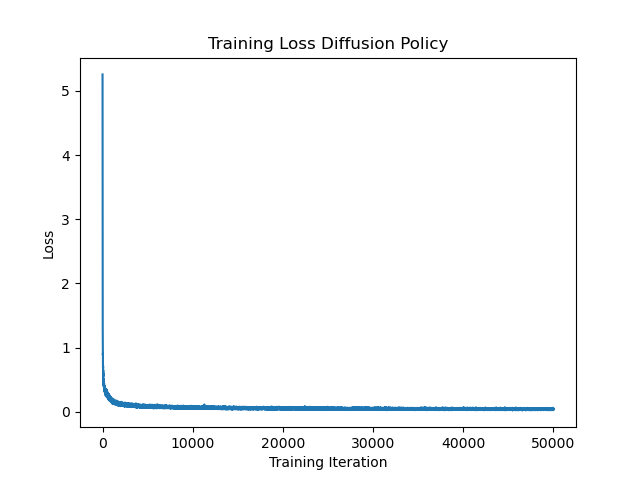
\includegraphics[width=33em]{code/results_diffusion/trial_2_BEST/diffusion_policy_loss.png}

            Final loss: 0.0469

            \end{solution}
            
            \end{tcolorbox}


\subsection*{2.3.2 Rewards Diffusion Policy (15 pts)}
\subsection*{2.3.2.1; 3 actions evaluated in a row (5 pts)}

avg trajectory time: \begin{tcolorbox}[fit,height=1cm, width=2cm, blank, borderline={1pt}{1pt},nobeforeafter]
    \begin{center}
    \vspace{3mm}
    \large{9.28 s}
    \end{center}
\end{tcolorbox}
mean: \begin{tcolorbox}[fit,height=1cm, width=2cm, blank, borderline={1pt}{1pt},nobeforeafter]
    \begin{center}
    \vspace{3mm}
    \large{183.5}
    \end{center}
\end{tcolorbox}
median: \begin{tcolorbox}[fit,height=1cm, width=2cm, blank, borderline={1pt}{1pt},nobeforeafter]
    \begin{center}
    \vspace{3mm}
    \large{261.1}
    \end{center}
\end{tcolorbox}
max: \begin{tcolorbox}[fit,height=1cm, width=2cm, blank, borderline={1pt}{1pt},nobeforeafter]
    \begin{center}
    \vspace{3mm}
    \large{266.1}
    \end{center}
\end{tcolorbox}
    \\

\subsection*{2.3.2.2; 2 actions evaluated in a row (5 pts)}

avg trajectory time: \begin{tcolorbox}[fit,height=1cm, width=2cm, blank, borderline={1pt}{1pt},nobeforeafter]
    \begin{center}
    \vspace{3mm}
    \large{14.51 s}
    \end{center}
\end{tcolorbox}
mean: \begin{tcolorbox}[fit,height=1cm, width=2cm, blank, borderline={1pt}{1pt},nobeforeafter]
    \begin{center}
    \vspace{3mm}
    \large{202.6}
    \end{center}
\end{tcolorbox}
median: \begin{tcolorbox}[fit,height=1cm, width=2cm, blank, borderline={1pt}{1pt},nobeforeafter]
    \begin{center}
    \vspace{3mm}
    \large{261.8}
    \end{center}
\end{tcolorbox}
max: \begin{tcolorbox}[fit,height=1cm, width=2cm, blank, borderline={1pt}{1pt},nobeforeafter]
    \begin{center}
    \vspace{3mm}
    \large{266.8}
    \end{center}
\end{tcolorbox}
    \\

    
\subsection*{2.3.2.3; 1 action evaluated in a row (5 pts)}

avg trajectory time: \begin{tcolorbox}[fit,height=1cm, width=2cm, blank, borderline={1pt}{1pt},nobeforeafter]
    \begin{center}
    \vspace{3mm}
    \large{31.22 s}
    \end{center}
\end{tcolorbox}
mean: \begin{tcolorbox}[fit,height=1cm, width=2cm, blank, borderline={1pt}{1pt},nobeforeafter]
    \begin{center}
    \vspace{3mm}
    \large{231.3}
    \end{center}
\end{tcolorbox}
median: \begin{tcolorbox}[fit,height=1cm, width=2cm, blank, borderline={1pt}{1pt},nobeforeafter]
    \begin{center}
    \vspace{3mm}
    \large{264.3}
    \end{center}
\end{tcolorbox}
max: \begin{tcolorbox}[fit,height=1cm, width=2cm, blank, borderline={1pt}{1pt},nobeforeafter]
    \begin{center}
    \vspace{3mm}
    \large{268.9}
    \end{center}
\end{tcolorbox}
    \\

\subsection*{2.3.3 GIF link Diffusion Policy (2 pts)}

\begin{tcolorbox}[fit,height=5em, width=40em, blank, borderline={1pt}{1pt},nobeforeafter]
            \begin{solution}
            \url{https://drive.google.com/file/d/10M9vmolRiQeCRepCSjUIh34KVuP8NDtT/view?usp=sharing}
            \end{solution}

\end{tcolorbox}
    
\subsection*{2.3.4 Compare diffusion policy and simple model runtime (written, 4 pts)}
\begin{tcolorbox}[fit,height=10em, width=40em, blank, borderline={1pt}{1pt},nobeforeafter]
            \begin{center}
            \begin{solution}
            \raggedright
BC/DAgger's SimpleNet gets an action from a single forward pass of a small MLP. 
The diffusion policy instead has to denoise its actions: every time it chooses actions it runs 30 sequential 
denoising steps, and each step is a full forward pass of a 6-layer transformer decoder. 

These steps cannot be parallelized since each depends on the previous one (sequentially)
On our CPU one SimpleNet call took $\approx$0.04\,ms versus $\approx$36.5\,ms for one 30-step 
diffusion sample ($\sim$1000$\times$ slower), which is why a diffusion trajectory takes 9--31\,s.

            \end{solution}
            \end{center}
            \end{tcolorbox}
\subsection*{2.3.5 Compare diffusion policy with different actions in a row runtime (written, 3 pts)}
\begin{tcolorbox}[fit,height=10em, width=40em, blank, borderline={1pt}{1pt},nobeforeafter]
            \begin{center}
            \begin{solution}
            \raggedright
Runtime is dominated by diffusion samples, which cost the same regardless of $N$ ($\approx$36.5\,ms each). 

Executing $N$ predicted actions per sample means an episode of $T$ steps needs only $\lceil T/N \rceil$ samples, 
so time per environment step scales as $1/N$, which results in 12.2\,ms ($N$=3), 18.3\,ms ($N$=2) and 38.0\,ms ($N$=1), 
The average trajectory times (9.28, 14.51, 31.22\,s) also depend on episode length (761, 791, 821 steps on average). 
            \end{solution}
            \end{center}
            \end{tcolorbox}

\clearpage

\end{document}